\chapter{Sequential Transport planning}

In this chapter, we describe the planning approaches we
selected, implemented, and tested.
We will attempt to leverage the acquired
Transport domain knowledge
while designing these approaches as much as possible.

\section{State-space forward planning}\label{forward-planning}

One of the most straightforward approaches to automated planning
is forward search \citep[Section~4.2]{Ghallab2004}
in state space (Figure~\ref{alg:forward-search}).
Although the algorithm is defined on a classical representation,
it can be used on any planning problem, where we can:
\begin{itemize}
\item determine if a state is a goal state or not;
\item iterate over all actions applicable to a state; and
\item compute a successor state by applying an action to the current state.
\end{itemize}
Forward search, despite its simplicity, is one of the most frequently
used in domain-independent planners.
There are two key steps of the algorithm, which
cause the most problems in practice: representing
the applicable actions (step 6) and choosing the
next action to apply (step 8).

\myalg{Forward Search}%
{%
\Input a planning problem in a classical representation $\mathcal{P} = (S, O, \gamma, s_0, g)$
\Output a plan $\pi$
\Function{Forward-Search}{$\mathcal{P}$}
\State $s \gets s_0$ 
\State $\pi \gets $ empty plan
\Loop
\If {$s$ satisfies $g$} \Return $\pi$ \EndIf
\State $A_s \gets \{a \,|\, o \in O$, $a$ is a ground instance of $o \;\&\; \mt{precond}(a) \mt{ is true in } s\}$
\If {$A_s = \emptyset$} \Return failure \EndIf
\State (nondeterministically) choose an action $a \in A_s$
\State $s \gets \gamma(s, a)$
\State $\pi \gets$ append $a$ to $\pi$
\EndLoop
\EndFunction
}%
{A forward search planning algorithm.}{A forward search planning algorithm for Transport. Adapted from \citet[Figure~4.1]{Ghallab2004}.}{forward-search}{bt}

Representing state transitions in step 6
is a technical problem of representing successor states
in state space search \citep[Section~3.2]{Russell1995}.
Due to limited memory,
applicable actions are grounded from operators
on demand, as are the corresponding successor states
\citep[Section~3.4]{Russell1995}.

The forward search algorithm, in its specified form, is nondeterministic.
If we knew which action to choose in step 8,
we would know how to solve the planning problem.
Since we generally do not know which action (state transition) to chose in a given state, the choice is usually delegated to a suitable
search algorithm, which makes the whole algorithm deterministic.


\subsection{Deterministic search algorithms}

State space search algorithms are a heavily studied area
of computer science and any reasonable search algorithm applied
to forward search will yield correct results.
Examples of such algorithms are Breadth-First Search (BFS), 
Depth-First Search (DFS), and many more \citep[Section~3.5]{Russell1995}.
The choice of a search algorithm greatly influence
the quality of resulting plans when applied to forward search.

As the sizes of planning problems grow,
choosing a search algorithm is even more crucial.
Several well-performing algorithms on small problems (like BFS)
exceed reasonable run times and become unusable for practical applications.
An important and practically useful search algorithm
withstanding larger problem sizes is the \textit{A$^{\kern-.15em*}$ algorithm} (Figure~\ref{alg:astar})
introduced in \citet{Hart1968}.

\myalg{Forward Search with A$^{\kern-.15em*}$}%
{%
\Input a classical planning problem $\mathcal{P} = (S, O, \gamma, s_0, g)$,
a consistent heuristic function $h$
\Output a plan $\pi$
\Function{Collect-Plan}{$s, \pi$}
\State $\pi' \gets $ empty list
\While{$s \neq \emptyset$}
	\State $(s', a) \gets \pi[s]$
	\State $\pi' \gets$ prepend $a$ to $\pi'$
	\State $s \gets s'$
\EndWhile
\State \Return $\pi'$
\EndFunction

\Function{Forward-Search-Astar}{$\mathcal{P}$}
\State $\pi \gets $ empty map, $f[*] \gets \infty$, $g[*] \gets \infty$, $o \gets \{s_0\}$, $c \gets \emptyset$
\State $\pi[s_0] \gets \emptyset$, 
$g[s_0] \gets 0$, $f[s_0] \gets h(s_0)$
\While{$o \neq \emptyset$}
\State $s \gets \mt{argmin}_{s \in o} f[s]$, $o \gets o \setminus \{s\}$, $c \gets c \cup \{s\}$
\If {$s$ satisfies $g$} \Return \Call{Collect-Plan}{$s$, $\pi$} \EndIf
\ForAll{actions $a \in$ \Call{Generate-Actions}{$s, \pi$}}
	\State $s' \gets \gamma(s, a)$
	\If{$s' \notin c$} \Comment{Not visited yet}
		\If{$s' \notin o$} $o \gets o \cup \{s'\}$ \Comment{Discovered a new state} \EndIf 
		\If{$g[s] + \mt{cost}(a) < g[s']$} \Comment{Found a better path}
			\State $\pi[s'] \gets (s, a)$
			\State $g[s'] \gets g[s] + \mt{cost}(a)$
			\State $f[s'] \gets g[s'] + h(s')$
		\EndIf
	\EndIf
\EndFor
\EndWhile
\Return failure
\EndFunction
}%
{A forward search planning algorithm using A$^{\kern-.15em*}$.}{A forward search planning algorithm using A$^{\kern-.15em*}$.
\textsc{Generate-Actions} is a function that produces actions applicable to the state $s$.}{astar}{tb}

A$^{\kern-.15em*}$ has many important properties. We pinpoint one important to us, namely its admissibility.
A search algorithm is \textit{admissible}
if it is guaranteed to find an optimal path from a state $s$
to a goal state $s_g$ for any state space \citep{Hart1968}.
A$^{\kern-.15em*}$ is admissible and optimal given an admissible heuristic.

An \textit{admissible} heuristic never overestimates
the true value it is approximating. During planning in state space,
when examining a state $s$, we want to estimate the total costs of the best
plan getting us to a goal state from state $s$. In other words, because we are
trying to minimize the total cost,
a planning heuristic $h: S \to \N_0$ is admissible if and only if $\forall s \in S : h(s) \leq h^*(s),$
where $h^*$ is the true total cost (in other words, the optimal heuristic). A similar definition is applicable for minimizing makespan in the temporal variant.

A slight modification of A$^{\kern-.15em*}{\kern-.30em,}$ called \textit{Weighted A$^{\kern-.15em*}$} \citep{Pohl1970},
tends to yield good quality plans in a shorter amount of time,
at the expense of
sacrificing admissibility. The only difference
when compared to A$^{\kern-.15em*}$ is that the heuristic $h(x)$
is substituted for $h_w(x) = w \cdot h(x),$
where $w \in \N_0$ is a weight constant. Choosing a weight greater
than 1 makes the heuristic inadmissible,
but guides the search towards a goal state faster.


\subsection{Heuristics for forward search in Transport}\label{seq-heuristics}

When designing a heuristic, we want to provide an estimate
of the total plan cost or makespan
that is as precise as possible, which
will help guide the search to a goal state as quickly as
possible.

We will now describe several heuristics for sequential
Transport using the state-variable representation.
In the following, the value of the $\mt{target(p)}$ function represents
the target location of a package $p$ in the set of packages $P$.

\subsubsection{Trivially admissible Transport heuristic}\label{sfa0}

The simplest domain-specific heuristic (apart from the zero heuristic $h_0 \equiv 0$) that is applicable to all variants of Transport
is one that counts the minimum number of \pickup{} and \drop{} actions
necessary to reach a goal state.
To obtain the correct count, we add 1 for each
package that is not yet at its destination (it will need to be dropped there) and another 1 for each package
that is, additionally, not in a vehicle (it will need to be picked up):

$$h'_{0}(s) = \sum_{\substack{
p \in P\\ \mt{at}(p) \neq \mt{target}(p)}} 1
+ \sum_{\substack{
p \in P\\ \mt{at}(p) \neq \mt{target}(p)\\
\mt{at}(p) \neq \mt{nil}}} 1.$$

The heuristic $h'_0$ is admissible, but it is practically unusable, as it
very poorly approximates 
the cost of the optimal remaining actions to a goal state
--- recall that costs of \drive{} actions are generally much higher than the costs of \pickup{} and \drop{} actions.

\subsubsection{Package distance heuristic}\label{sfa1}

In \texttt{transport-strips}, the only thing we want is to deliver packages to their destinations. Therefore, a straightforward heuristic is one that calculates the length of a shortest
path of each package to its destination and sums the lengths for all packages.
To make the heuristic more precise, we can add the
value of $h'_0$ to it, as the \pickup{} and \drop{}
actions also have to occur in the optimal plan:
$$h_1 = h'_0 + \sum_{p \in P} \mt{spd}(location(p), target(p)),$$
where the $location: P \to L$ function,
with values in the set of all locations $L$, is defined as
$$location(p) = \begin{cases} 
   \mt{at}(p) & \text{if } \mt{at}(p) \neq \mt{nil}\\
   \mt{at}(\mt{in}(p)) & \text{else}.
  \end{cases}$$
The location of a package will is, therefore, defined
as the location it is at, or, if it is in a vehicle,
the location of the vehicle.
The function $\mt{spd}: L \times L \to \N_0$ represents
the shortest path distance between the two locations.

This heuristic is definitely not optimal, meaning that there are states,
where we will need to add actions to reach a goal state with a higher total cost than the value of the heuristic in that state.

However, it is important to note, the heuristic
is not even admissible, so its value might sometimes overestimate the total cost needed.
To see why, let us consider a network with just two locations $A$ and $B$.
A vehicle of capacity 2 and two packages are located at $A$ and both packages want to be
transported to $B$. The road between $A$ and $B$ is symmetric and has length
of a 100. It is trivial to see that the optimal plan consists of two \pickup{} actions,
followed by a \drive{} and two \drop{} actions. This plan has a total cost of $2+100+2=104$,
but the heuristic would estimate that we need actions
that cost $204$.

\subsubsection{Minimum spanning tree marking heuristic}\label{sfa2}

A different extension of the $h'_0$ heuristic
is the heuristic $h_2$ defined below, based
on finding the shortest paths on a \textit{minimum spanning tree} (MST).
Using an MST calculated using the algorithm presented in \citet{Kruskal1956}, we can solve one of the largest problems with $h_1$,
namely that we count an excessive amount of \drive{} actions
for packages to their targets.
For each package, we will calculate
shortest path distances only on the MST.
Also, we will not calculate any edge twice --- we will mark
the edge when it happens to be part of a shortest path and
after marking edges of all shortest paths,
we sum the lengths of the marked edges.
In the same way as with $h_1$, we add the value of $h'_0$ to
the sum.

Do note that this heuristic is yet again inadmissible:
let the road network be a circle of $n$ locations with
roads of lengths $1, 2, \ldots, n$ assigned clockwise.
An MST on this network consists of all roads except the road
with length $n$, lets denote the road $r = (A, B) \in L^2$.
Now, assume there is a package located at $A$ with a target
location of $B$ and a vehicle also located at $A$.
The optimal plan is obviously to pick up the package at $A$,
drive along road $r$ to $B$, and drop the package there.
The plan has a cost of $n+2$. The $h_2$ heuristic's estimate
in the initial state is $$h_2(s_0) = 2 + \sum_{i=1}^{n-1} i = \frac{n^2}{2} - \frac{n}{2} + 2,$$
which is evidently greater than $n+2$ for $n > 3$.

\subsubsection{Package and vehicle distance heuristic}\label{sfa3}

As an extension of the package distance heuristic,
we will also add the distance of the nearest vehicle for
each package:
$$h_3 = h_1 + \sum_{p \in P} \min_{v \in V} \mt{spd}(location(p), \mt{at}(v)),$$
where $V$ is the set of all vehicles.
As follows from the inadmissibility of $h_1$, $h_3$
is also inadmissible and nonoptimal.

\subsubsection{Package or vehicle distance heuristic}\label{sfa4}

A variation on the package and distance heuristic
is one that does not sum, but instead takes
the minimum distances.
Specifically, for each package, the minimum
is taken from the distance to its target location,
distance to the nearest vehicle,
and the distance to the nearest package:
\begin{align*}
h_4 = h'_0 + \sum_{p \in P} \min\lbrace
&\mt{spd}(location(p), target(p)),
\min_{v \in V} \mt{spd}(location(p), \mt{at}(v)),\\
&\min_{\substack{p' \in P\\p' \neq p}} \mt{spd}(location(p), location(p'))\rbrace.
\end{align*}
We will now show a few properties of this heuristic.
\begin{thm}
The heuristic $h_4$ is admissible for sequential Transport problems.
\end{thm}
\begin{proof}
Let $s$ be a state such that $h_4(s) > h^*(s)$,
where $h^*$ is a function of the real distance to the nearest goal state.
State $s$ is not a goal state, because for all goal states $s'$
it holds that
$h_4(s') = 0 = h^*(s'),$ due to all packages being at their target locations.
Let $s_g$ be the nearest goal state to $s$.

Because $h_4(s) > h^*(s)$, there exists a finite plan $\pi$ from $s$ that ends in $s_g$,
such that the total cost of $\pi$ is less than $h_4(s)$.
Using induction, we prove that for all intermediate states $s'$ of $\pi$,
$h_4(s') \leq h^*(s'),$ which is a contradiction with $h_4(s) > h^*(s)$,
as $s$ is the initial state of $\pi$.

Let $n$ be the number of actions in $\pi$.
If $n=0$, $s$ is a goal state and, therefore, $h_4(s) = 0 = h^*(s)$.

Let us number all intermediate states of $\pi$ in reverse order: $$\{s = s_k, s_{k-1}, \ldots, s_2, s_1, s_0 = s_g\}.$$
Now, assume that our conjecture holds for the last $n < k$ states.
We will prove that it then also holds for the last $n+1$ states.
Let us denote the transition action between $s_{n+1}$ and $s_{n}$ as $a$.

If $a$ were a \pickup{} or \drop{} action, only the value of $h'_0$
would have changed, and by at most 1 in the correct direction,
which means that $h_4(s_{n+1}) \leq h^*(s_{n+1}).$

If $a$ were a \drive{} action
\TODO{finish proof}.
\end{proof}

However, the $h_4$ heuristic is not consistent. Assume the following road network (Figure~\ref{fig:heursit}):
$$\{\{A, B, 1\}, \{B, C, 2\}, \{B, D, 2\}\},$$
where $\mt{at}(v) = A$, $\mt{at}(p_1) = C,$ and $\mt{at}(p_2) = D$
hold in the initial state $s_0$.
The target of $p_1$ is $D$ and the target of $p_2$ is $C$.
The value
$$h_4(s_0) = 3+3+4 = 10$$ is greater than the cost
of the applicable \drive{} action for vehicle $v$ from $A$ to $B$
added to the heuristic value in the updated state:
$$cost(a) + h_4(s') = 1 + (2+2+4) = 9.$$
The heuristic is also not optimal, as is evident from the same
example situation (for $s_0$, the optimal plan is of length $13$).

\begin{figure}[tb]
\centering
\includegraphics[width=0.3\textwidth]{../imga/heursit}
\caption{Visualization of the counterexample road network
for consistency of $h_4$.}
\label{fig:heursit}
\end{figure}

\subsubsection{General marking heuristic}\label{sfa5}

The heuristic $h_5$ is a generalization of the MST marking heuristic $h_2$. We calculate $h_5$ in the exact same way by marking roads,
except for
using an MST --- instead, the whole graph is used.
We also mark roads on the shortest path from each package to the nearest
vehicle or package or target location, depending on which is nearer (similar
to the package or vehicle distance heuristic).
Shortest path ties are broken arbitrarily.
Do note that if a package is loaded in a vehicle, no roads are marked for it.

The described heuristic is not optimal, but it is admissible.
Both properties hold because $\forall s \in S : h_5(s) \leq h_4(s)$ holds.

\begin{thm}
The heuristic $h_5$ is consistent for sequential Transport problems.
\end{thm}
\begin{proof}
Let $s$ be a state and $s_g$ the nearest goal state.
We will (equivalently) show that $h_5(s) \leq h_5(s') + cost(a),$ where
$s' = \gamma(s, a)$ for all applicable $a \in A$.

If $a$ is a \pickup{} or \drop{} action,
no road will be marked because of the package that was picked up/dropped,
due to the nearest vehicle being present at the same location.
The markings of other packages do not change, because
the vehicle picking up or dropping the package does not move
and shortest distances are calculated to packages and vehicles.
Therefore, even if the minimum was previously hit at the package that was
picked up, it would be hit at the vehicle that was picking up
the package anyway (analogously for the \drop{} action).
Therefore, the inequality holds trivially, because $h_5(s) = h_5(s') - 1$ (for \drop{})
or $h_5(s) = h_5(s') + 1$ (for \pickup{}), and the cost of $a$ is 1.

Assume $a$ is a \drive{} action of the vehicle $v$.
We can ignore all packages that are loaded onto the vehicle,
as they only contribute to the value with 1 for the \drop{} action
that has to happen. That does not change by appending a \drive{} action.
\TODO{finish proof}
\end{proof}


\subsubsection{Summary}

In our tests, we found that
the heuristics $h_0$, $h'_0$, $h_1$, and $h_2$
were too simple for practical usage.
The $h_3$ heuristic, while having no significant
theoretical properties performs surprisingly well in practice.
The $h_4$ heuristic on the other hand, while being admissible, does not
perform well empirically.
Due to its consistency, the $h_5$ heuristic has the best theoretical properties out of all the discussed heuristics and also
performs well in practice.
We will include planners utilizing the $h_3$ and $h_5$ heuristics
in our final evaluation (Chapter~\ref{experiments}).








\subsection{Sequential Forward A$^{\kern-.15em*}$}\label{sfa}

\textit{Sequential Forward A$^{\kern-.15em*}$} (SFA) is a planner for sequential Transport based on forward search using A$^{\kern-.15em*}$ (Figure~\ref{alg:astar}).
It utilizes most of the domain knowledge described
in Section~\ref{domain-info} and~\ref{datasets}
to prune the search space as much as possible
without sacrificing admissibility.

However, domain knowledge alone does not
prune away enough search space to
generate plans efficiently.
With the addition of 
heuristics
from Section~\ref{seq-heuristics}
implementations of the planner become reasonably useful
on practical problems, as will be demonstrated
later during experimental evaluation.

A variant of SFA, 
\textit{Weighted Sequential Forward A$^{\kern-.15em*}$} (WSFA)
swaps A$^{\kern-.15em*}$ search for Weighted A$^{\kern-.15em*}$ in the SFA planner.

\subsection{Meta-heuristically weighted SFA$^{\kern-.15em*}$}\label{msfa}

\textit{Meta-heuristically weighted SFA$^{\kern-.15em*}$} (MSFA) is
a meta-planner built on top of a WSFA planner with
a given heuristic.

Given two hyperparameters $\alpha \in [0, 1]$ and $w_0 \in [1, \infty)$,
it runs the WSFA planner with the weight $w \gets w_0$,
waits for the planner to find a plan,
and then (exponentially) decays the 
weight of the heuristic function: $w \gets \max(1, \floor*{\alpha \cdot w}).$
Do note that this entails a change of values in the $f$ map
of forward search with A$^{\kern-.15em*}$.

Even though this meta-planning approach breaks
admissibility guarantees, it works very well on
practical problems, even the larger ones.



















\section{Ad-hoc planning}\label{ad-hoc}

An approach that domain-independent planners by definition cannot utilize
is ad-hoc planning. We propose several
ad-hoc planners that generate decent quality plans very fast,
although they are usually suboptimal.
This becomes an advantage mainly when dealing with very large
problems or time-constrained planning,
like in the agile track of IPC.

\subsection{Randomized Restart Planning}\label{rand-restart}

We will now describe a family of planners which we will refer to as \textit{Randomized Restart} planners.
Each of these planners essentially performs the same algorithm (Figure~\ref{alg:rand-restart}),
with minor tweaks. The motivation
behind the algorithm is that the ``hardest'' part of Transport planning
is choosing where to drive with what vehicle.

\myalg{Randomized Restart planning}%
{%
\Input a Transport problem in a classical representation $\mathcal{P} = (S, O, \gamma, s_0, g)$
\Output a plan $\pi$
\Function{Randomized-Restart}{$\mathcal{P}$}
\State $\pi \gets $ empty plan, $\Pi \gets \infty$
\While{cancel not requested} \Comment{Canceled by an external request}
\State $s \gets s_0$, $\pi' \gets $ empty plan
\While{$s$ doesn't satisfy $g \And score(\pi') < \Pi$}
\State $A \gets $ \Call{Generate-Drive-Sequence}{$s$}
\ForAll{action $a \in A$} \Comment{Apply all actions to the state}
\State $s \gets \gamma(s, a)$
\EndFor
\If{$s = \emptyset$} \textbf{break} \Comment{At least one $a \in A$ was not applicable}
\EndIf
\State $\pi' \gets $ append all $a \in A$ to $\pi'$
\EndWhile
\If{$s$ satisfies $g \And score(\pi') < \Pi$}
\State $\pi \gets \pi'$, $\Pi \gets score(\pi')$ \Comment{Update the best plan}
\EndIf
\EndWhile
\State \Return $\pi$
\EndFunction
}%
{A Randomized Restart planning algorithm.}{A Randomized Restart planning algorithm. The \textsc{Generate-Drive-Sequence} function
generates a partial plan beginning in state $s$.
The exact definition of the function
depends on the specific algorithm variant as described in Section~\ref{rand-restart}.}{rand-restart}{tb}

The algorithm essentially does domain-dependent plan space planning
by iteratively adding sequences of \drive{} actions
intertwined with \pickup{} and \drop{} actions
until all packages are delivered.
To do all of this at speed, the vehicle used for the given sequence
is usually chosen randomly, as are the packages that are picked up and dropped along the driving path.
The biggest advantage, however, is gained by precomputing
a matrix of shortest paths and always using those to drive to the
selected locations.

Our randomized restart planners will generate many suboptimal plans,
but by always keeping a copy of the so far best found plan,
we can prune away the current partial plan if it becomes
worse than the best plan after adding a sequence.
Afterwards, we simply restart
from the initial state and iteratively generate a new candidate plan.
We utilize domain knowledge in all the planners,
for example by not picking up packages that are at their destination,
and most of the other insights discussed in Section~\ref{domain-info}.

\subsubsection{Randomized Restart From Location Planner}\label{rrfl}

In each iteration of the before mentioned algorithm,
the Randomized Restart From Location planner (RRFL)
randomly chooses a vehicle and a location.

It adds \drive{} actions along the shortest path
to that location and greedily picks up as many packages as
its capacity allows.
It then calculates the optimal
path through all the picked up package target locations,
by trying the shortest paths through all possible permutations
of the locations.
Finally, it adds the appropriate \drive{} and \drop{} actions.

\subsubsection{Randomized Restart On Path Planner}\label{rrop}

The Randomized Restart On Path planner (RROP),
randomly chooses a vehicle
and a package that fits into the vehicle.
It then calculates the shortest path from the vehicle
to the package
and the shortest path from the package to its target location.
Afterwards, it finds all packages on that have current and target locations on the path, taking into account the direction of driving.
It then tries all combinations of
those packages that do not make the vehicle become
overcapacitated over the whole course
of the path,
to find the combination that minimizes the minimum
free capacity over the course of the path.
If there are several such combinations, it minimizes the
maximum package drop location index in the path.
If there are still several combinations, it chooses one arbitrarily.
Finally, it adds the appropriate \drive{} and \drop{} actions.

\subsubsection{Randomized Restart On Path Nearby Planner}\label{rropn}

The Randomized Restart On Path Nearby planner (RROPN)
is a slight modification of RROP.
It first chooses a package randomly and then,
based on a probability $\varepsilon \in [0, 1]$,
either chooses a random vehicle that the package fits into,
or the nearest such vehicle.
The rest of the algorithm is identical to RROP.
The probability $\varepsilon$ is a hyperparameter,
which in our experiments is fixed to $0.2$,
which means that the probability of selecting the nearest vehicle is 80\%.

\subsubsection{Randomized Restart Around Path Nearby Planner}\label{rrapn}

Another randomized restart planner that is built on top of RROPN,
is the Randomized Restart Around Path Nearby planner (RRAPN).
It uses the same vehicle and package selection,
but it changes the way packages on the path are chosen to be loaded
onto the vehicle.

We still load as many packages that are completely on the path
as possible, using the same selection mechanism as in RROPN.
Additionally, for each package we precalculate
the location on the path that is closest to its target,
limited to locations after the package was picked up
in the correct driving direction.
Finally, we plan the \pickup{} and \drop{} actions of the
packages that greedily fit into the vehicle and
have the smallest precalculated distance to their target.

\subsubsection{Randomized Backtrack Around Path Nearby Planner}\label{rbapn}

We also developed a backtracking variant of RRAPN
called Randomized Backtrack Around Path Nearby (RBAPN).
Instead of choosing random vehicles and packages
it backtracks over the choices it makes,
guaranteeing to find an optimal
plan in the subspace of plans
generated by adding such action sequences as described in
the section about RRAPN. This approach is very
time-consuming and not practically usable.

\subsubsection{Randomized Restart Around Path Distribution Planner}\label{rrapd}

Another variant of RRAPN, the
Randomized Restart Around Path Distribution planner (RRAPD),
changes the vehicle choice of inherited from RROPN.
Instead of using a biased coin flip based on the $\varepsilon$
hyperparameter, RRAPN samples the vehicle
from a discrete probability distribution
obtained by applying the \textit{softmax} function on the distances of vehicles to the selected package:
\begin{align*}
\varphi'_i &= \frac{1}{\mt{spd}(location(p), \mt{at}(v_i)) + 1}\\
\varphi_i &= \frac{\exp(\varphi'_i/T)}{\sum_{j = 1}^{|V|} \exp(\varphi'_j/T)}
\end{align*}
The value $\varphi_i$ is the resulting probability of each vehicle $v_i \in V = \{v_1, v_2, \ldots, v_n\}$.
The hyperparameter $T \in (0, \infty)$ is the \textit{temperature}
of the softmax. If set to higher values than 1, it
evens out the distribution --- higher probabilities shrink
and smaller probabilities become larger.
As $T$ grows large, the distribution will resemble a uniform distribution.
If $T$ is set to lower values, the distribution will prefer larger values.
In our experiments, we used a fixed $T = 0.1$, to prefer the nearest vehicles.

\subsubsection{Sumamry}

In our tests, the implementations
of RRFL, RROP, and RROPN have empirically shown
lesser performance than RRAPN and RRAPD.
RRAPD, however, performs worse than RRAPN on
average.
As mentioned previously, RBAPN is unusable on larger
problems due to catastrophic run time in practice.
We will evaluate the Nearby planner
of the Randomized Restart Around Path
kind in our experiments in Chapter~\ref{experiments},
as they produce good quality plans in a very short time
even for larger problem instances.

All planners of the Randomized Restart family
are suboptimal, not only meaning that they sometimes produce
suboptimal plans, but also that for some problems,
even the best plan they can produce will be suboptimal.
This is easiest to prove for each planner individually,
by constructing a counterexample for a corner
case of the 
greedy
choices
the planners make.



























\comment{
\section{Formulating Transport as a CSP}\label{csp-approach}

When discussing related works, we mentioned the Vehicle Routing Problem (Section~\ref{vrp}) and its straightforward
formulation as a Constraint Satisfaction Problem. Utilizing CSPs has been useful
for planning in the past \citep[Section~8.7]{Ghallab2004}
and we will attempt to use domain-specific knowledge to improve upon the standard, domain-independent
formulation.

\subsection{Na{\"{i}}ve CSP formulation}

We will now formulate a sequential Transport (Section~\ref{transport-strips}) problem as a CSP (Section~\ref{csp}) using the na{\"{i}}ve encoding provided in \citet[Section~8.3]{Ghallab2004}.


TODO{explain the model + constraints}


However, using that strategy, our problems ``blow up'' in size --- as is expected due
to the different complexities of planning versus solving CSPs \citep[Section~8.3.2]{Ghallab2004}. To visualize the difference in our case, we have constructed a state space estimation table (Table~\ref{tab:csp-trivial}) for conversions of two sample sequential Transport problems.

TODO{recalculate + verify numbers}

\begin{table}[tb]
\begin{center}
\begin{tabular}{l||rr}
\textbf{Features / estimates} & \textbf{p01} & \textbf{p20} \\ 
\midrule
\midrule
\textbf{Best-known plan length} & 6 & 351 \\ 
\textbf{Vehicles} & 2 & 4 \\ 
\textbf{Vehicle variables} & 14 & 1 408 \\ 
\textbf{Packages} & 2 & 20 \\ 
\textbf{Package variables} & 14 & 7 040 \\ 
\textbf{Locations} & 5 & 60 \\ 
\textbf{Roads} & 12 & 256 \\
\textbf{Max capacity} & 4 & 4 \\ 
\midrule
\textbf{Ground Drive actions} & 168 & 360 448 \\ 
\textbf{Ground PickUp actions} & 140 & 1 689 600 \\ 
\textbf{Ground Drop actions} & 140 & 1 689 600 \\ 
\midrule
\textbf{Planning variables total} & 48 & 10 207 \\ 
\textbf{Grounded actions total} & 448 & 1 189 838 848 \\ 
\textbf{Search Space Estimate} & $\approx 1.1 \cdot 10^{52}$ & $\approx 1.4 \cdot 10^{27 952}$ \\ % https://www.wolframalpha.com/input/?i=(245120%5E351)+*+4%5E1408+*+60%5E1408+*+1468%5E7040
\end{tabular}
\end{center}
\caption[Search space approximations for a na{\"{i}}ve CSP encoding.]{CSP Search space approximations for the \textit{p01} and \textit{p20} problems from the \textit{seq-sat} track of IPC 2008, using the general and domain-independent encoding from \citet[Section~8.3]{Ghallab2004}.}
\label{tab:csp-trivial}
\end{table}

The first section of the table (rows 1--7) contains problem-specific constants.
The two calculated values in that section, \textit{Vehicle variables} and \textit{Package variables} are the numbers of variables generated for the respective
object by grounding it for every intermediate plan state (before and after applying an action). Therefore, the value is equal to the number of vehicles/packages of the problem
multiplied by the set plan length + 1 (each state corresponds to the state before applying an action + the last state).

In the second section (rows 8--10), we estimate the number of ground actions
Step 1 from \citet[Section~8.3.1]{Ghallab2004} will generate.
We calculate the number of \pickup{} and \drop{} actions the CSP encoding will generate
as $$(\mt{length(plan)} + 1) \cdot \mt{\#vehicles} \cdot \mt{\#locations} \cdot \mt{\#packages},$$
effectively counting all ground planning operators of the problem. Similarly,
the number of \drive{} actions is calculated as
$$(\mt{length(plan)} + 1) \cdot \mt{\#vehicles} \cdot \mt{\#roads},$$
which is more efficient than the na{\"{i}}ve way of
counting all
$$(\mt{length(plan)} + 1) \cdot \mt{\#vehicles} \cdot \mt{\#locations}^2$$
actions.

As we can see from the third section of the table, the number of variables
(planning variables and ground actions) is not extremely high
--- the problem is that the variables have very large domains,
which makes the CSP problem exponentially larger \citep[Section~8.3.2]{Ghallab2004}.
We calculated the \textit{Search Space Size Estimate} (SSE) as
\begin{align*}
\mt{SSE} =\; &\mt{\#ground\_actions}^{l-1} & \textit{\footnotesize select ground actions for the plan}\\
&\cdot \mt{\#capacities}^{l \cdot \mt{\#vehicles}} & \textit{\footnotesize select capacities for vehicle variables}\\
&\cdot \mt{\#locations}^{l \cdot \mt{\#vehicles}} & \textit{\footnotesize select locations for vehicle variables}\\
&\cdot (\mt{\#locations} + \mt{\#vehicles})^{l \cdot \mt{\#pkg}}, & \textit{\footnotesize select locations/vehicles for package variables}
\end{align*}
where we set $l := \mt{length(plan) + 1}$.
For comparison to the SSEs in the last table row, 
the estimated number of atoms in the universe is generally estimated to be about $4 \cdot 10^{80}$.

\subsection{Domain-dependent CSP representation}\label{csp-custom-repr}

We will now devise a different CSP representation for sequential Transport.
While not improving upon the search space estimates of the na{\"{i}}ve formulation
in a theoretical sense, we will describe a slightly more complex
and less general
CSP model that enables us to explore fewer states.

Using OptaPlanner and its shadow variable concept \citep[Section~4.3.6]{DeSmet2017}, we will model our Transport problem without keeping explicit track of capacities,
vehicle and package locations, and ground actions, all of which will be implicitly managed by OptaPlanner, or inferred in the case of capacity and actions.
This means we will reduce the memory overhead, maintaining the same expressive power
and hopefully not enlarge the processing time too much.

TODO{Describe the specific representation after it is polished in the code}

TODO{recalculate + verify numbers}

\begin{table}[tb]
\begin{center}
\begin{tabular}{l||rr}
\textbf{Features / estimates} & \textbf{p01} & \textbf{p20} \\ 
\midrule
\midrule
\textbf{Best-known plan length} & 6 & 351 \\ 
\textbf{Vehicles} & 2 & 4 \\ 
\textbf{Vehicle shadow vars} & 14 & 1 408 \\
\textbf{Packages} & 2 & 20 \\ 
\textbf{Package shadow vars} & 14 & 7 040 \\
\textbf{Locations} & 5 & 60 \\
\textbf{Roads} & 12 & 256 \\
\textbf{Max capacity} & 4 & 4 \\ 
\midrule
\textbf{Ground Drive actions} & 24 & 1024 \\ 
\textbf{Ground PickUp actions} & 20 & 4800 \\ 
\textbf{Ground Drop actions} & 20 & 4800 \\ 
\midrule
\textbf{Planning variables total} & 48 & 10 207 \\ 
\textbf{Grounded actions in step} & 64 & 10 624 \\ 
\textbf{Action type orderings} & 2 187 & $\approx 8.8 \cdot 10^{167}$ \\ 
\textbf{Search Space Estimate} & $\approx 1.5 \cdot 10^{14}$ & $\approx 2.0 \cdot 10^{637}$ \\
\end{tabular}
\end{center}
\caption[Search space approximations for a domain-dependent CSP representation.]{CSP Search space approximations for the \textit{p01} and \textit{p20} problems from the \textit{seq-sat} track of IPC 2008, using a custom domain-dependent CSP representation for Transport sequential.}
\label{tab:csp-custom}
\end{table}

Using the domain-dependent representation specified, we are now able to construct
a search space estimate table for the same Transport problems (Table~\ref{tab:csp-custom}). 
Do note, that this table cannot be compared directly to the previous one,
because it hides the shadow variable management overhead.
Also, while the table rows look similar, sections 2 and 3 are calculated
differently. The ground action counts in section 2 are not multiplied by $\mt{length(plan)} + 1$
as done previously, because we only represent them once, not at every plan state.
The total number of grounded actions is the same, but they are not explicitly represented as variables. The Search Space size Estimate is therefore calculated differently:
\begin{align*}
\mt{SSE} =\; &3^{\mt{length(plan)} + 1} & \textit{\footnotesize select the action type of each action}\\
&\cdot \mt{\#ground\_actions}^{l-1}. & \textit{\footnotesize select the specific ground action}
\end{align*}
For comparison to the na{\"{i}}ve encoding SSEs which going from the p01 problem to p20 grow by a logarithmic factor of approximately $538$,
whereas the domain-dependent ones only grow by approximately $46$,
which is a huge improvement.

Given the search space reduction, we will now attempt to use this representation
for constructing a CSP-based planner.

\subsection{CSP-based planner}\label{csp-planner}

TODO{try to run a CSP in OptaPlanner to solve this and compare results, using Section~\ref{csp-custom-repr}}

TODO{Advantages and shortcommings of a CSP-based planner}

}